\chapter{AND, OR, NOT gates}
%\ref{sec:background}.

\section{Aim}
%\label{sec:objectives}
	To verify and interpret the logic and truth table for AND, OR, NOT gates using Resistor Transistor Logic (RTL), Diode Resistance Logic (DRL) and Transitor Logic (TL) 

\section{Apparatus}
%\label{sec:objectives}
	\begin{itemize}
		\tightlist
		\item Kit for realization of gates
		\item Connecting Leads
	\end{itemize}

\section{Circuits}
	

\section{Theory}
	Logic gates are the basic building blocks of any digital system. Logic gates are electronic circuits having one or more than one input and only one output. The relationship between the input and the output is based on a certain logic. Based on this, logic gates are named as:
	\begin{enumerate}
		\tightlist
		\item AND gate
		\item OR gate
		\item NOT gate
		\item NAND gate
		\item NOT gate
		\item Ex-OR gate
		\item Ex-NOR gate
	\end{enumerate}
	
	\subsection{AND gate}
	The AND gate is an electronic circuit that gives a high output $(1)$ only if all its inputs are high. A dot $(.)$ is used to show the AND operation i.e. $A.B$ or can be written as $AB$.
	\begin{align*}
		Y &= A . B
	\end{align*}
	A simple 2-input logic AND gate can be constructed using RTL (Resistor-Transistor-Logic) switches connected together as shown below with the inputs connected directly to the transistor bases. Both transistors must be saturated “ON” for an output at $Q$.
	\begin{figure}[ht]
		\centering 
		\subfloat[Symbol]
		{
			\begin{circuitikz} \draw
				(0,0) node[and port] (myand1) {}
				(myand1.in 1) node[anchor=east] {A}
				(myand1.in 2) node[anchor=east] {B}
				(myand1.out) node[anchor=west] {Y}
				;
			\end{circuitikz}
			\label{fig:and_symbol}
		}	
		\hfill
		\subfloat[Truth Table]
		{
			\begin{tabular}{|c|c|c|}
				\hline
				\multicolumn{2}{|c|}{Input} & Output \\
				\hline
				$A$ & $B$ & $Y=A.B$ \\
				\hline
				0 & 0 & 0 \\
				\hline
				0 & 1 & 0 \\
				\hline
				1 & 0 & 0 \\
				\hline
				1 & 1 & 1 \\
				\hline
			\end{tabular}
			\label{fig:and_table}
		}
		\hfill
		\subfloat[RTL Design]{
			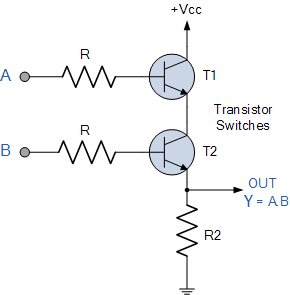
\includegraphics[width=0.25\textwidth,valign=c]{img/exp1/fig1}
			\label{fig:and_circuit}
		}
		\caption{\textit{AND gate}}
	\end{figure}
	
	
	\subsection{OR gate}
		The OR gate is an electronic circuit that gives a high output $(1)$ if one or more of its inputs are high. A plus $(+)$ is used to show the OR operation.		
		\begin{align*}
			Y &= A + B
		\end{align*}		
		OR gate can be realized by DRL (Diode-Resistance-Logic) or by TTL (Transistor-Transistor-Logic). Presently, we will learn how to implement the OR gate using DRL (Diode-Resistance-Logic). To realise OR gate, we will use a diode at every input of the OR gate. The anode part of diode is connected with input while the cathode part is joined together and a resistor, connected with the cathode is grounded. In this case, we have taken two inputs which can be seen in the circuit below.
		
		When both the inputs are at logic $0$ or low state then the diodes $D_1$ and $D_2$ become reverse biased. Since the anode terminal of diode is at lower voltage level than the cathode terminal, so diode will act as open circuit so there is no voltage across resistor and hence output voltage is same as ground. When either of the diodes is at logic $1$ or high state then the diode corresponding to that input is forward bias. Since this time anode is at high voltage than cathode therefore current will flow through forward biased diode and this current then appears on resistor causing high voltage at output terminal also. Hence at output we get high or logic $1$ or $+5V$. So, if any or both inputs are high, the output will be high or $1$.
		\begin{figure}[ht]
			\centering 
			\subfloat[Symbol]
			{
				\begin{circuitikz} \draw
					(0,0) node[or port] (myand1) {}
					(myand1.in 1) node[anchor=east] {A}
					(myand1.in 2) node[anchor=east] {B}
					(myand1.out) node[anchor=west] {Y}
					;
				\end{circuitikz}
				\label{fig:or_symbol}
			}	
			\hfill
			\subfloat[Truth Table]
			{
				\begin{tabular}{|c|c|c|}
					\hline
					\multicolumn{2}{|c|}{Input} & Output \\
					\hline
					$A$ & $B$ & $Y=A+B$ \\
					\hline
					0 & 0 & 0 \\
					\hline
					0 & 1 & 1 \\
					\hline
					1 & 0 & 1 \\
					\hline
					1 & 1 & 1 \\
					\hline
				\end{tabular}
				\label{fig:or_table}
			}
			\hfill
			\subfloat[DRL Design]{
				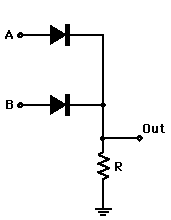
\includegraphics[width=0.25\textwidth,valign=c]{img/exp1/fig2}
				\label{fig:or_circuit}
			}
			\caption{\textit{OR gate}}
		\end{figure}
	
	\subsection{NOT gate}
	The NOT gate is an electronic circuit that produces an inverted version of the input at its output. It is also known as an inverter. If the input variable is $A$, the inverted output is known as $NOT A$. This is also shown as $A'$ or $A$ with a bar over the top, as shown at the outputs.
	\begin{align*}
		Y &= \overline{A}
	\end{align*}
	NOT gate can be realized through transistor.The input is connected through resistor $R_2$ to the transistor’s base. When no voltage is present on the input, the transistor turns off. When the transistor is off, no current flows through the collector-emitter path. Thus, current from the supply voltage ($V_{cc}$) flows through resistor $R_1$ to the output. In this way, the circuit’s output is high when its input is low.
	
	When voltage is present at the input, the transistor turns on, allowing current to flow through the collector-emitter circuit directly to ground. This ground path creates a shortcut that bypasses the output, which causes the output to go low.
	
	In this way, the output is high when the input is low and low when the input is high.
	\begin{figure}[ht]
		\centering 
		\subfloat[Symbol]
		{
			\begin{circuitikz} \draw
				(0,0) node[not port] (mynot) {}
				(mynot.in) node[anchor=east] {A}
				(mynot.out) node[anchor=west] {Y}
				;
			\end{circuitikz}
			\label{fig:not_symbol}
		}	
		\hfill
		\subfloat[Truth Table]
		{
			\begin{tabular}{|c|c|}
				\hline
				Input & Output \\
				\hline
				$A$ & $Y = \overline{A}$ \\
				\hline
				0 & 1 \\
				\hline
				1 & 0 \\
				\hline
			\end{tabular}
			\label{fig:not_table}
		}
		\hfill
		\subfloat[TL Design]{
			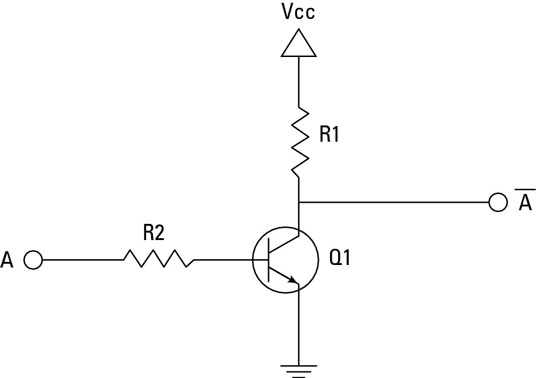
\includegraphics[width=0.25\textwidth,valign=c]{img/exp1/fig3}
			\label{fig:not_circuit}
		}
		\caption{\textit{NOT gate}}
	\end{figure}
		
\section{Procedure}
	\subsection{AND gate}
		\begin{figure}[ht]
			\centering 
			\subfloat[Simulator 1]{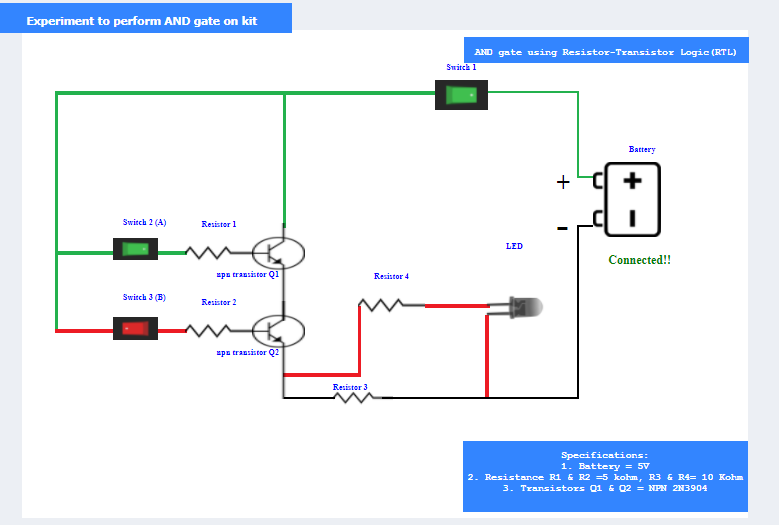
\includegraphics[width=0.45\textwidth,valign=c]{img/exp1/fig4}
				\label{fig:and_sim:1}}	
			\hfill
			\subfloat[Simulator 2]{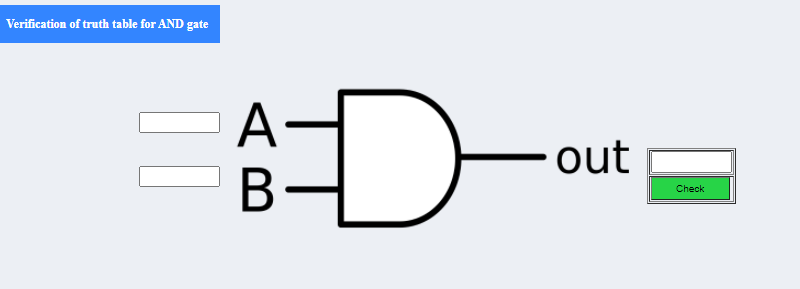
\includegraphics[width=0.4\textwidth,valign=c]{img/exp1/fig5}
				\label{fig:and_sim:2}}			
			\caption{\textit{Simulator for realizing circuit for AND gate}}
		\end{figure}
		\subsubsection{Simulator 1}
			\begin{enumerate}
				\tightlist
				\item Connect the supply(+5V) to the circuit.
				\item Press the switches for inputs "A" and "B".			
				\item The bulb does not glow if any one or both the switches (2 and 3) are OFF and glows only if both the switches (2 and 3) are ON.
				\item Repeat step-2 and step-3 for all state of inputs.
			\end{enumerate}
		\subsubsection{Simulator 2}
			\begin{enumerate}
				\tightlist
				\item Enter the Boolean input "A" and "B".
				\item Enter the Boolean output for your corresponding inputs.
				\item Click on "Check" Button to verify your output.			
			\end{enumerate}	

	\subsection{OR gate}
		\begin{figure}[ht]
			\centering 
			\subfloat[Simulator 1]{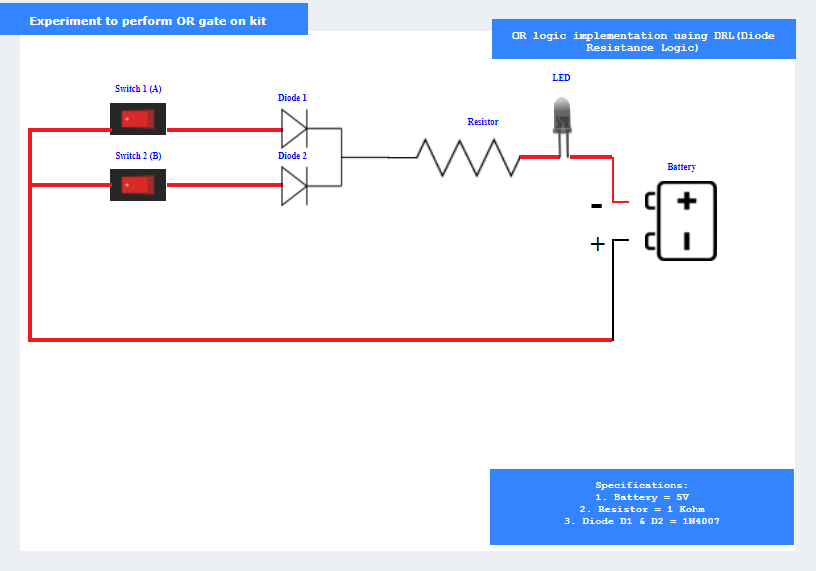
\includegraphics[width=0.45\textwidth,valign=c]{img/exp1/fig6}
				\label{fig:or_sim:1}}	
			\hfill
			\subfloat[Simulator 2]{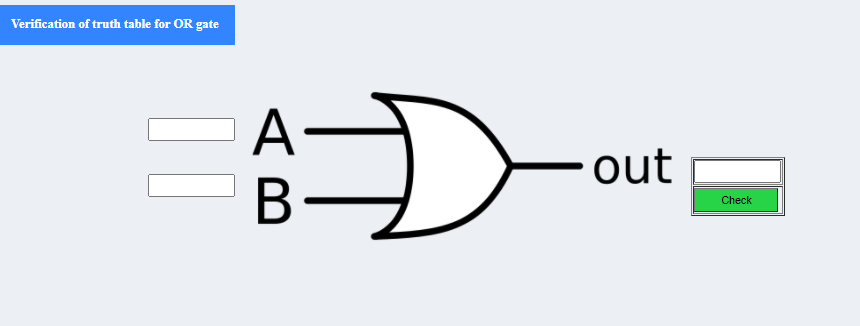
\includegraphics[width=0.4\textwidth,valign=c]{img/exp1/fig7}
				\label{fig:or_sim:2}}			
			\caption{\textit{Simulator for realizing circuit for OR gate}}
		\end{figure}
		\subsubsection{Simulator 1}
			\begin{enumerate}
				\tightlist
				\item Connect the supply(+5V) to the circuit.
				\item Press the switches for inputs "A" and "B".			
				\item The bulb glows if any one or both the switches are ON else it won't glow.
				\item Repeat step-2 and step-3 for all state of inputs.
			\end{enumerate}
		\subsubsection{Simulator 2}
			\begin{enumerate}
				\tightlist
				\item Enter the Boolean input "A" and "B".
				\item Enter the Boolean output for your corresponding inputs.
				\item Click on "Check" Button to verify your output.			
			\end{enumerate}

	\subsection{NOT gate}
		\begin{figure}[ht]
			\centering 
			\subfloat[Simulator 1]{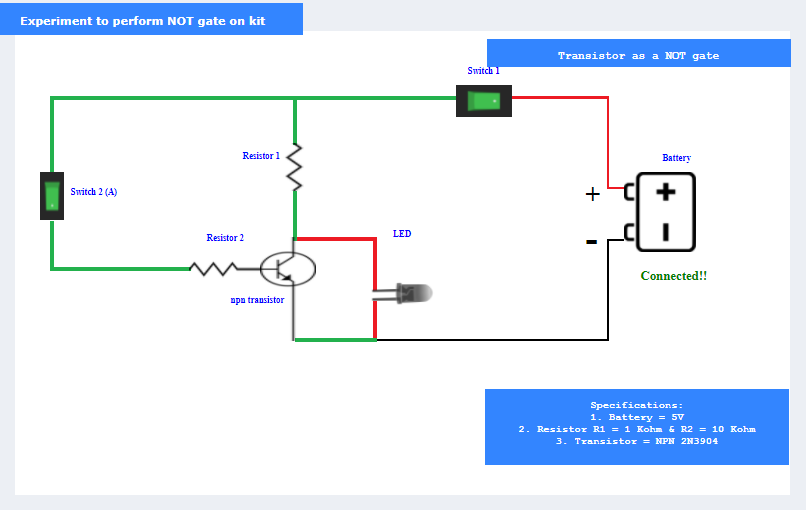
\includegraphics[width=0.45\textwidth,valign=c]{img/exp1/fig8}
				\label{fig:not_sim:1}}	
			\hfill
			\subfloat[Simulator 2]{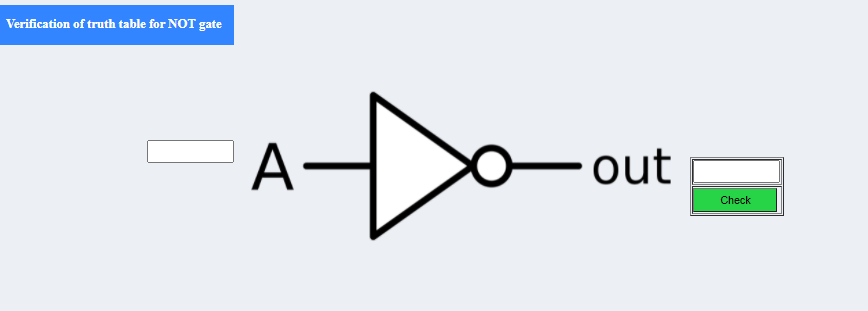
\includegraphics[width=0.4\textwidth,valign=c]{img/exp1/fig9}
				\label{fig:not_sim:2}}			
			\caption{\textit{Simulator for realizing circuit for NOT gate}}
		\end{figure}
		\subsubsection{Simulator 1}
			\begin{enumerate}
				\tightlist
				\item Connect the supply(+5V) to the circuit.
				\item Press the switch 1 to connect battery to the circuit.
				\item Press the switch 2 for input "A".
				\item The bulb glows if switch 2 is OFF else it won't glow.
			\end{enumerate}
		\subsubsection{Simulator 2}
			\begin{enumerate}
				\tightlist
				\item Enter the Boolean input "A".
				\item Enter the Boolean output for your corresponding input.
				\item Click on "Check" Button to verify your output.			
			\end{enumerate}

\section{Observations}
	\subsection{AND gate}
			\begin{figure}[ht]
				\centering 
				\subfloat[Either of the Inputs OFF, LED is OFF]{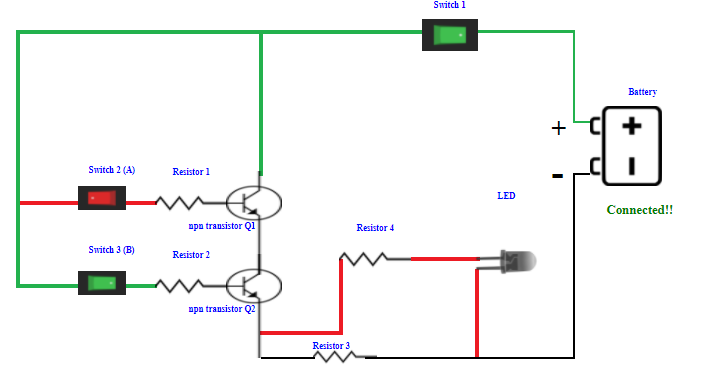
\includegraphics[width=0.45\textwidth,valign=c]{img/exp1/fig10}
					\label{fig:and_obs:1}}	
				\hfill
				\subfloat[Both Inputs ON, LED is ON]{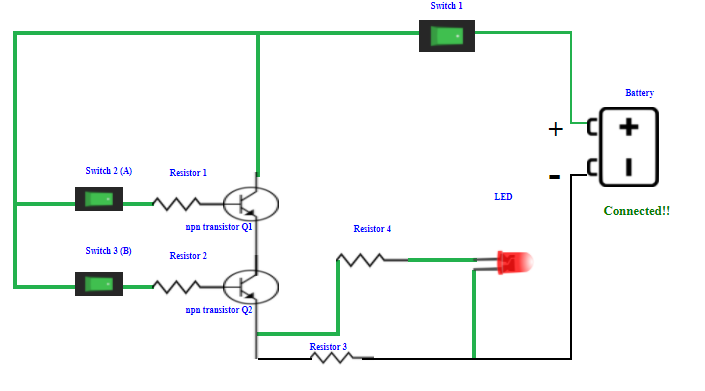
\includegraphics[width=0.45\textwidth,valign=c]{img/exp1/fig11}
					\label{fig:and_obs:2}}			
				\caption{\textit{Observations for different Input Values}}
			\end{figure}
			\begin{figure}[h]
				\centering
				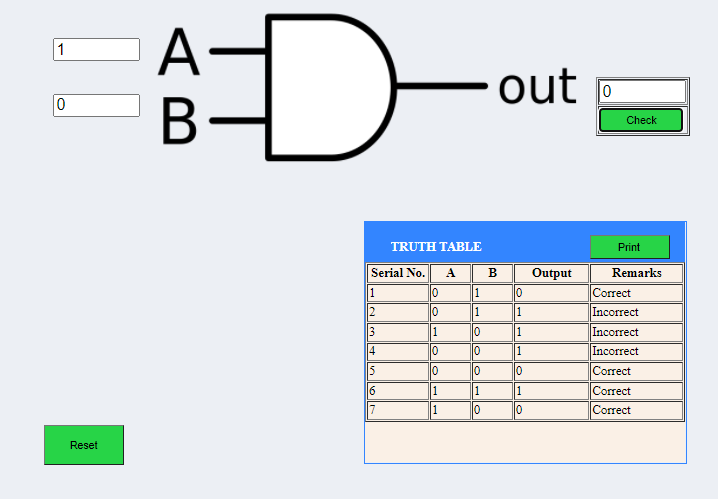
\includegraphics[width=0.85\linewidth]{img/exp1/fig12}
				\caption{\textit{Observations for verification of Truth Table of the AND gate}}
				\label{fig:and_obs_2}
			\end{figure}

\pagebreak
	\subsection{OR gate}
			\begin{figure}[ht]
				\centering 
				\subfloat[Either of the Inputs ON, LED is ON]{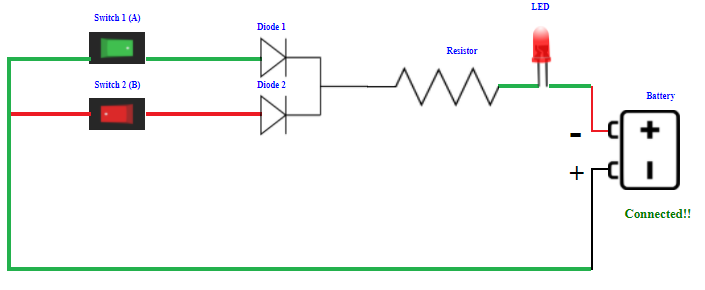
\includegraphics[width=0.45\textwidth,valign=c]{img/exp1/fig13}
					\label{fig:or_obs:1}}	
				\hfill
				\subfloat[Both Inputs OFF, LED is OFF]{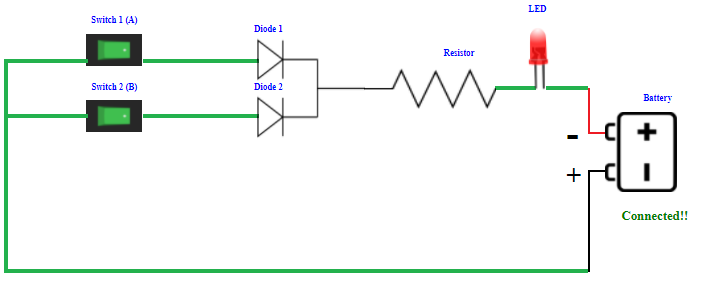
\includegraphics[width=0.45\textwidth,valign=c]{img/exp1/fig14}
					\label{fig:or_obs:2}}			
				\caption{\textit{Observations for different Input Values}}
			\end{figure}
			\begin{figure}[h]
				\centering
				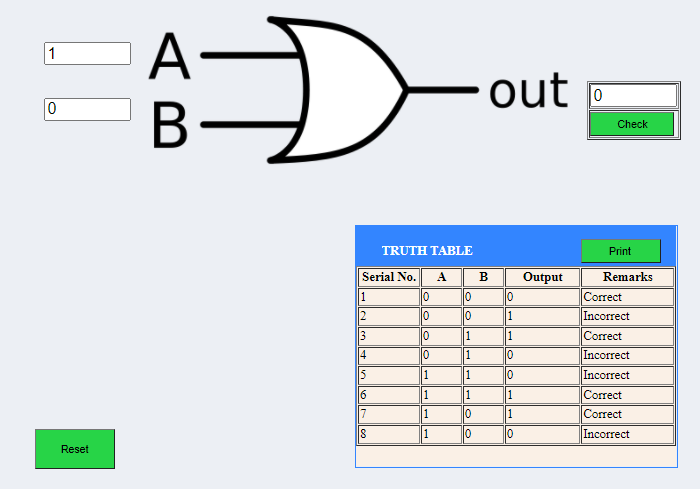
\includegraphics[width=0.85\linewidth]{img/exp1/fig15}
				\caption{\textit{Observations for verification of Truth Table of the OR gate}}
				\label{fig:or_obs_2}
			\end{figure}

\pagebreak
	\subsection{NOT gate}
			\begin{figure}[ht]
				\centering 
				\subfloat[Input is ON, Output is OFF]{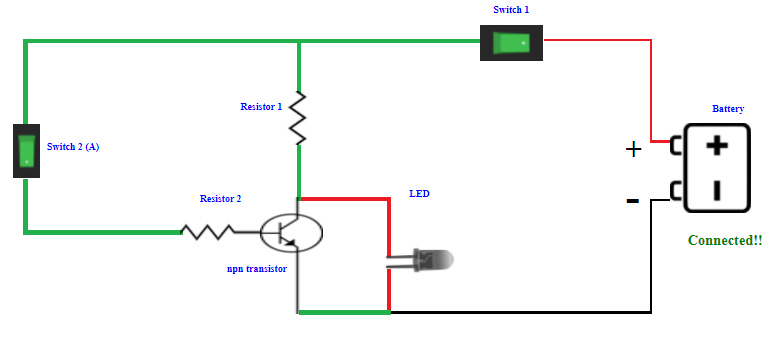
\includegraphics[width=0.45\textwidth,valign=c]{img/exp1/fig16}
					\label{fig:not_obs:1}}	
				\hfill
				\subfloat[Input is OFF, Output is ON]{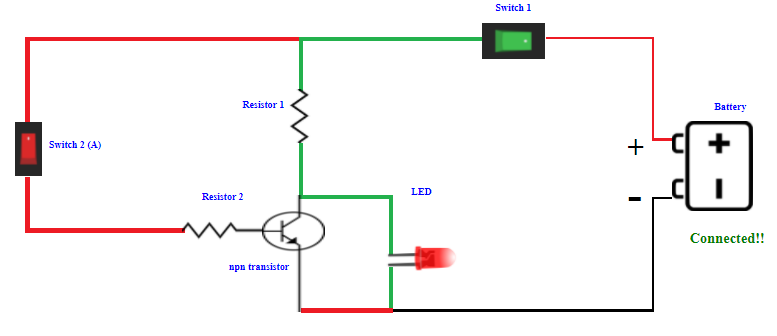
\includegraphics[width=0.45\textwidth,valign=c]{img/exp1/fig17}
					\label{fig:not_obs:2}}			
				\caption{\textit{Observations for different Input Values}}
			\end{figure}
			\begin{figure}[h]
				\centering
				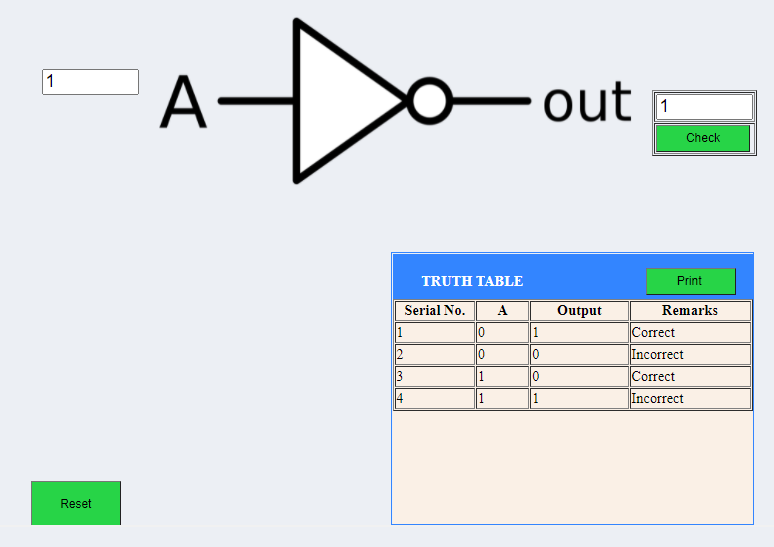
\includegraphics[width=0.85\linewidth]{img/exp1/fig18}
				\caption{\textit{Observations for verification of Truth Table of the NOT gate}}
				\label{fig:not_obs_2}
			\end{figure}
			
\section{Precautions}
	\begin{enumerate}
		\tightlist
		\item Make the connections when power supply is OFF.
		\item Ensure that the connections are tight.
		\item Change the status of inputs only when power supply is OFF.
	\end{enumerate}